\subsection{Dubbi esistenziali}
Su scala macroscopica la materia è continua, ma per spiegare alcune proprietà dobbiamo assumere sia discontinua, costituita da atomi, i quali possono avere carica e quindi esistono gli ioni. Inoltre esistono le molecole.

Cerchiamo ora di spiegare:
\begin{enumerate}
    \item Come sono fatti gli atomi;
    \item Perché e come si legano insieme producendo molecole;
    \item Perché abbiamo atomi che portano cariche se fondamentalmente dovrebbero essere neutri;
    \item Se quando formiamo molecole, esse abbiano o meno relazioni con gli atomi costituenti (cioè se hanno proprietà che dipendono da essi).
  \end{enumerate}
  
  \subsection{Onde elettromagnetiche}
Le onde elettromagnetiche sono costituite da due vettori: campo elettrico $\vec{E}$ e campo magnetico $\vec{H}$, perpendicolari tra loro che oscillano nel tempo. La velocità dell'onda è la velocità della luce $c$.

\vspace{0.2cm}\textbf{DEF} Ampiezza: altezza massima di un'onda rispetto alla direzione di propagazione. 

\vspace{0.2cm}\textbf{DEF} Frequenza ($\nu$): numero di oscillazioni per unità di tempo. È inversamente proporzionale alla lunghezza d'onda ($\lambda$): $\lambda\nu=c$, cioè $\lambda=c/\nu$.

\subsection{La luce: onda o corpuscolo?}
Nella fisica classica moto ondulatorio e moto dei corpi sono due teorie a sè stanti, ognuna con le proprie leggi.
In particolare per i fenomeni ondulatori esiste il fenomeno dell'interferenza, che consiste nella sovrapposizione di due onde.
Per la luce ci sono due ipotesi:
\begin{itemize}
  \item  La teoria di Newton: la luce ha natura corpuscolare, cioè è formata da fotoni;
  \item  La teoria di Huygens: la luce è un fenomeno ondulatorio, priva di massa e dotata solo di energia.
\end{itemize}
\subsection{Fenomeni che supportano la natura ondulatoria della luce (e della materia)}
\begin{itemize}
  \item  Diffrazione: è un fenomeno associato alla deviazione della traiettoria di propagazione delle onde quando queste incontrano un ostacolo sul loro cammino.
  \item  Interferenza: due o più onde elettromagnetiche si sovrappongono in un punto dello spazio in modo costruttivo (si intensificano) o distruttivo (si indeboliscono fin quando si annullano a vicenda).
  \item  Riflessione: un'onda che si propaga lungo l'interfaccia tra differenti mezzi, cambia direzione a causa di un impatto con un materiale riflettente.
  \item  Rifrazione: deviazione subita da un'onda che ha luogo quando questa passa da un mezzo ad un altro otticamente differenti nel quale la sua velocità di propagazione cambia.
\end{itemize}
\subsection{Esperimento di Young (1801)}
Rafforza la teoria di Huygens. Si pone una sorgente luminosa dietro una superficie con una fenditura. La fenditura diventa a sua volta sorgente di fronti d'onda sferici (diffrazione). Oltre questa superficie ce n'è un'altra con 2 fenditure che a loro volta diventano sorgenti di fronti d'onda sferici. Proiettando il risultato su uno schermo si ottengono zone luminose e zone buie alternate. Se la luce da origine alla diffrazione, allora deve avere natura ondulatoria e non corpuscolare.

\subsection{Conseguenze della luce come onda}
Se la luce è un'onda, allora la sua energia è proporzionale a $E^2$ ed $H^2$, cioè dipende dalla ampiezza e non dalla sua frequenza. 

Ciò fu messo in crisi dalle evidenze sperimentali sulla radiazione emessa da un corpo caldo: quando si riscalda un corpo, esso riemetterà tale energia sotto forma di radiazione \comment{(per raffreddarsi) mi pare inutile scriverlo fai te pd negridimerda} con frequenza che \textbf{dipende} dalla sua temperatura e dalla sua composizione chimica. Ma ciò non dovrebbe accadere se l'energia non dipende dalla frequenza! Dunque la temperatura del corpo è legata alla frequenza della radiazione che emette (e quindi la sua energia). 

Un corpo nero è un oggetto ideale capace di assorbire radiazione incidente di qualunque frequenza\footnote{Per conservazione dell'energia emette anche radiazione a tutte le frequenze.}. La migliore approssimazione reale di corpo nero è una sfera di nerofumo con un piccolo foro in cui inviamo radiazione. Essa verrà riflessa varie volte all'interno riscaldando la sfera. Aumentando la temperatura, gli atomi si eccitano ed emettono radiazione diseccitandosi. Classicamente avremmo dovuto osservare uno spettro di emissione su tutte le frequenze fino all'UV, invece si osserva che vengono emesse solo alcune frequenze. Inoltre all'aumentare della temperatura l'intensità diventa maggiore e il picco di emissione si sposta a frequenze maggiori. 

Il massimo dello spettro è legato alla temperatura dalla legge di Wien 
$$T\cdot\lambda_{max}= \text{cost}= 2.8977\cdot 10^{-3} \; \rm m \cdot K$$

%oh merda a fine pagina 59 pure tu non chiudi una parentesi, tutto il resto del corso di chimica è solo una parentesi

\subsection{Quantizzazione: equazione di Planck}%devo andare mi sto pisciando addosso
Se un pezzo di metallo è riscaldato ad alta temperatura, la radiazione elettromagnetica emessa ha frequenza dipendente dalla temperatura. 

\begin{figure}[htp]
  \centering
  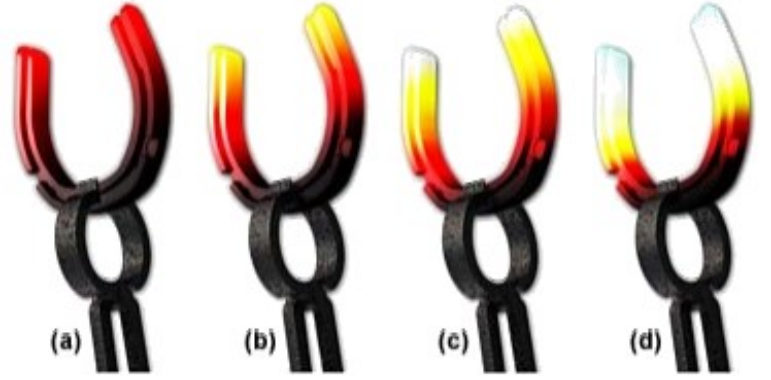
\includegraphics[width=8cm]{immagini/ferro_incandescente.png}
\end{figure}

A temperature inferiori il colore è rosso sbiadito, ma con l'aumentare della temperatura diventa rosso più acceso. Gli occhi rilevano la radiazione emessa nella regione visibile dello spettro elettromagnetico. Sebbene non visibile, anche UV ed infrarossi sono emessi dal metallo caldo. All'aumentare della temperatura, l'intensità massima si sposta verso lunghezze d'onda inferiori (cioè UV). Alla fine del 1800, gli scienziati non erano in grado di spiegare la relazione tra intensità e lunghezza d'onda della radiazione emessa da un oggetto caldo (radiazione di corpo nero). Le teorie disponibili a quel tempo predicevano che l'intensità aumenta col diminuire della lunghezza d'onda, invece di raggiungere un massimo e poi diminuire. Questa situazione era nota come catastrofe ultravioletta perché la predizione falliva nella regione UV. Max Planck offrì una spiegazione per la catastrofe ultravioletta: la radiazione elettromagnetica emessa è originata da vibrazione di atomi dell'oggetto riscaldato. Propose che ogni atomo avesse una frequenza fondamentale di oscillazione e che gli atomi potessero oscillare solo a questa frequenza o ad un multiplo di essa. Quindi la radiazione emessa ha solo certe energie, data dalla equazione 
$$E=nh\nu \qquad n\in\mathbb{N},n \neq 0 $$
Con $\nu$ frequenza della radiazione ed h costante di Planck.

Per la prima volta si parla di quantizzazione: etichettato $h\nu$ un pacchetto di energia, l'energia varrà $1, 2, \dots, n$ volte questa quantità con n numero intero. Si dice quindi che n quantizza la quantità di energia.
Dunque mentre prima tutte le energie potevano essere  assunte, ora si parla di energie permesse: un atomo o i suoi elettroni non possono possedere qualunque valore di energia, ma solo alcuni. L'energia quindi non è più continua ma quantizzata.

Planck assunse che ci deve essere una distribuzione di vibrazioni di atomi in un oggetto, cioè alcuni atomi hanno alte frequenze, altri intermedi ed altri basse. I pochi atomi con alta frequenza di vibrazione sono responsabili di alcuna luce, ad esempio UV e quelli con frequenza bassa emettono nell'infrarosso. Tuttavia, la maggior parte della luce deve venire dagli atomi che oscillano a frequenze intermedie (che sono di più). Cioè lo spettro di luce è emesso con un massimo di intensità alle lunghezze d'onda intermedie, in accordo con evidenze sperimentali. L'intensità non diventa maggiore all'avvicinarsi nella regione UV.
L'aspetto chiave del lavoro di Planck è l'introduzione di energie quantizzate basate sull'equazione $E=h\nu$.

Quando osserviamo un oggetto di un certo colore, ciò che succede nei suoi atomi è che i loro elettroni si sono eccitati passando ad un valore più alto di energia e, diseccitandosi, hanno emesso proprio la differenza di energia tra quel livello e lo stato fondamentale, a cui dall'eq. di Planck corrisponde una certa frequenza e quindi un certo colore. In altre parole, i livelli energetici degli atomi sono quantizzati, per cui i loro elettroni non possono avere qualsiasi valore energetico ma solo alcuni detti \textit{stati permessi}.

Le energie delle radiazioni elettromagnetiche si distribuiscono secondo la legge di distribuzione di Boltzmann:

$$P\propto e^{{-\frac{nh\nu}{KT}}}$$

\subsection{Effetto fotoelettrico}
Altro fenomeno che non si riusciva a spiegare con la teoria classica.

Esso consiste nell'emissione di elettroni da parte di una superficie metallica quando questa viene colpita da una radiazione elettromagnetica avente opportuna frequenza. Gli elettroni emessi si chiamano fotoelettroni.
Se la radiazione ha bassa frequenza non osserviamo fotoemissione, ma facendo crescere la frequenza ci accorgiamo che a un certo punto tale fenomeno inizia a verificarsi. Da ciò si deduce che c'è una soglia minima da superare affinché si emettano elettroni. Inoltre se aumenta l'intensità della radiazione incidente l'energia degli elettroni emessi non cambia, aumenta solo il loro numero. Se invece aumenta la frequenza della radiazione l'energia cinetica dei fotoelettroni emessi aumenta.

Einstein ebbe l'intuizione di usare l'espressione di Planck e di applicare il principio di conservazione dell'energia: se inviamo una certa quantità di energia al materiale, affinché avvenga fotoemissione essa deve essere almeno uguale alla quantità necessaria per vincere la forza di attrazione elettrone-nucleo (energia di legame), che costituisce la soglia di emissione. Dopodiché, usando l'espressione di Planck fu chiaro che, essendo l'energia funzione della frequenza, se cambia la frequenza della radiazione incidente cambia anche l'energia. Usata una parte dell'energia per vincere l'energia di legame, il resto si trasforma in energia cinetica del fotoelettrone emesso.
Pertanto all'aumentare della frequenza aumenta l'energia cinetica dell'elettrone.

In generale quindi il pacchetto di energia dovrà essere uguale a un valore costante $\Phi$ detto \textbf{potenziale di estrazione} e l'eventuale eccesso di energia del pacchetto si trasformerà in energia cinetica del fotoelettrone emesso.
$$h\nu=\Phi+\frac{1}{2}mv^2 \qquad E_k=h\nu-h\nu_0$$
$\nu_0$ è detta frequenza di soglia.

A questo punto Einstein affermò che la radiazione che arriva su una superficie deve essere composta da particelle, le quali arrivano sulla superficie e ad essa trasferiscono energia: ecco l'idea dei fotoni, particelle prive di massa.

Si torna quindi all'ipotesi di Newton.

Ma se la luce è fatta di particelle, come mai osserviamo fenomeni ondulatori?
\subsection{Spettro di emissione}
Supponiamo di eccitare singoli atomi, inviando varie energie. Questi ne assorbiranno alcune soltanto, e nella fase di diseccitazione le riemetteranno. Si osserva che emettono righe ben precise, a lunghezze d'onda ben precise. L'insieme di queste righe costituisce lo spettro di emissione di un atomo.

\begin{figure}[htp]
  \centering
  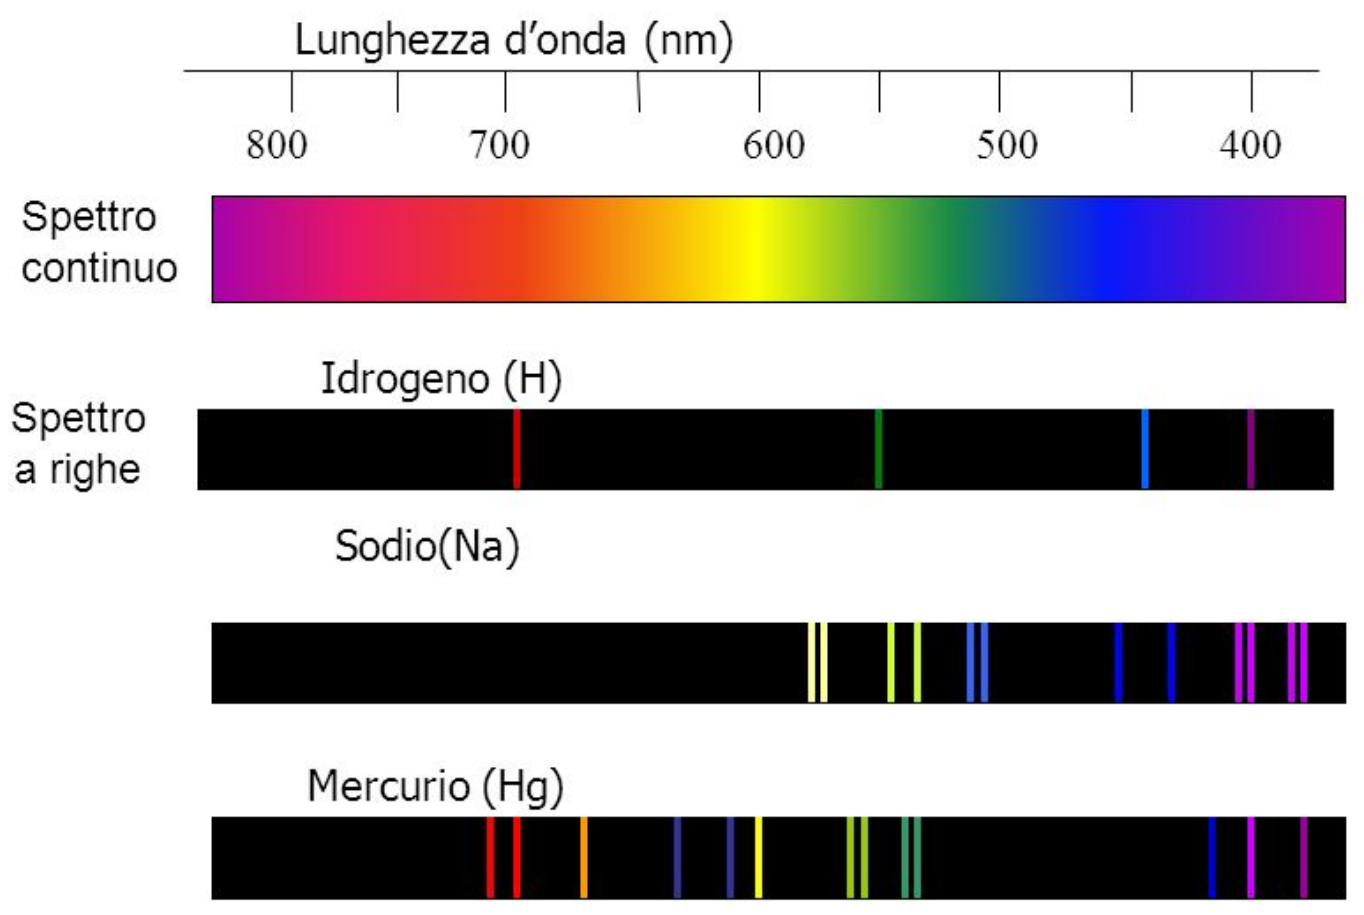
\includegraphics[width=8cm]{immagini/spettro_emissione.png}
\end{figure}

Il fatto che ci siano più righe implica che ci siano più stati permessi per l'elettrone.
\subsection{Esperimento di Rutherford}
Che tipo di modello atomico (struttura atomica) dobbiamo allora considerare per razionalizzare le emissioni?

Inizialmente si pensava al modello a panettone di Thomson, poi si passò a quello di Rutherford.

Rutherford bombardò una lamina d'oro dallo spessore di un migliaio di atomi con raggi $\alpha$ (ioni \ce{He^2+}). Egli osservò che la maggior parte di queste particelle attraversava indisturbata la lamina, come se non avessero incontrato ostacoli.
Qualche particella invece subiva deviazioni molto grandi, e in qualche caso tornava persino indietro. Allora suppose che la maggior parte della materia fosse costituita da spazio vuoto e che la maggior parte della massa \comment{c'è scritto materia ma non ha un cazzo di senso usare due volte la stessa parola} fosse concentrata in una piccolissima porzione dello spazio, quindi nella maggior parte dei casi le particelle passano indisturbate, ma nel caso in cui colpiscano la materia subiscono grandi deviazioni. Ecco l'idea della materia come spazio vuoto.

Rutherford propose per primo che l'atomo fosse costituito da un nucleo localizzato al centro, dove era concentrata tutta la massa, mentre gli elettroni dovevano essere a grande distanza dal nucleo stesso.
\subsection{L'atomo di Bohr (modello ragionevole)}
Bohr fece una prima ipotesi, con cui riuscì a spiegare lo spettro di emissione dell'atomo di idrogeno.

Egli pensò che l'atomo avesse una struttura simile a quella del sistema planetario, con un nucleo centrale dove c'è la massa e gli elettroni che ruotano a grande distanza dal nucleo.

Il nucleo è fatto da protoni (le cariche positive) e un certo numero di neutroni che schermano i protoni fra di loro (se questi non ci fossero i protoni sarebbero instabili perché hanno la stessa carica e si respingerebbero). Gli elettroni infine rendono neutro l'atomo.

Tuttavia, se l'elettrone ruota attorno al nucleo secondo la fisica classica deve compiere un moto a spirale fino a cadere sul nucleo perdendo energia, ovvero secondo il modello classico il modello degli elettroni che ruotano attorno al nucleo non era stabile.

Bohr allora ipotizzò una condizione di equilibrio: un elettrone che ruota a una certa distanza dal nucleo subisce una forza centrifuga che tende ad allontanarlo dal nucleo, ma siccome sull'elettrone agisce anche la forza di attrazione nucleo-elettrone affinché il sistema sia stabile queste due quantità devono essere uguali.
$$F_c=\frac{m_ev^2}{r} \quad \text{(Forza centrifuga)} \qquad F_{el}=-\frac{e^2}{r^2} \quad \text{(Forza elettrica)}$$
$$\text{Condizione di equilibrio} \quad F_c=-F_{el} \implies \frac{m_ev^2}{r}=\frac{e^2}{r^2}$$
In queste condizioni l'elettrone è in uno stato stazionario.

Condizioni di Bohr:
\begin{enumerate}
  \item L'elettrone in un atomo deve occupare stati stazionari: non può avere qualunque energia, ma solo quella permessa da tali stati. Quando l'elettrone si trova in uno di questi, non emette né assorbe energia. Se inviamo una radiazione possiamo far sì che l'elettrone assorba esattamente la differenza di energia tra questi due stati, ma deve essere proprio quella: se ne inviamo meno non basta, se ne inviamo di più non serve.
  Facendo così l'elettrone transiterà da uno stato ad uno a più alta energia.
  \item In questi stati l'elettrone si muove in orbite circolari attorno al nucleo.
  
  Ci sono due errori in questa frase:

  $\bullet$ Il termine "orbite": l'elettrone non si muove in un'orbita. Se così fosse, potremmo conoscere con esattezza posizione e velocità in qualunque istante. Si parlerà infatti di orbitale.

  $\bullet$ Il termine "circolare": se ci fosse una traiettoria, sarebbe ellittica.
  \item Gli stati permessi sono quelli in cui il momento angolare dell'elettrone è un multiplo intero di $\hbar=h/2\pi$. In altre parole si quantizza il momento angolare dell'elettrone. 
\end{enumerate}
Matematicamente, la quantizzazione del momento angolare si esprime come
$$m_evr=n\frac{h}{2\pi}\ \xrightarrow[\; \text{elevo al quadrato} \;]{} \ m_e^2v^2r^2=n^2\frac{h^2}{4\pi^2}$$
Ricaviamo il raggio
$$r^2=n^2\frac{h^2}{4\pi^2m_e^2v^2}$$
Sostituiamo nella condizione di equilibrio e ricaviamo il raggio:
$$\frac{m_ev^2}{r}=\frac{e^24\pi^2m_e^2v^2}{m^2h^2}\ \rightarrow\ r=\frac{n^2h^2}{4\pi^2e^2m_e}$$
Esso è detto \textit{raggio delle orbite di Bohr}.

Tale relazione ci dice che i raggi delle orbite sono quantizzati da n, ossia il modello di Bohr ci dice che oltre al momento angolare dell'elettrone, anche il raggio dell'orbita che esso segue è quantizzato. Si deduce quindi che l'elettrone non può stare a qualunque distanza dal nucleo, ma solo a distanze ben precise che dipendono da n.

\vspace{0.2cm}Ragioniamo ora sull'energia.

L'energia totale di un sistema è dato dalla somma di energia cinetica e potenziale\footnote{Essa è negativa, perché siamo in uno stato legato, cioè l'elettrone è legato all'atomo.}, che per un elettrone legato all'atomo si esprime come
$$E=E_{cin} + E_{pot}=\frac{1}{2}m_ev^2 - \frac{e^2}{r}$$
Dalla condizione di equilibrio segue che
$$m_ev^2=\frac{e^2}{r}\ \implies\ E=\frac{1}{2}\frac{e^2}{r} - \frac{e^2}{r}=- \frac{e^2}{2r}$$
Sostituendo il valore di $r$ si ha
$$E=-\frac{2\pi^2m_ee^4}{n^2h^2}$$
Cioè anche l'energia è quantizzata e dipende da $n$. Per esattezza si ha
$$E=-\frac{2.18\cdot10^{-18}}{n^2} \; \text{J}
=-\frac{13.6}{n^2} \; \rm eV$$
\subsection{Problemi insiti nel modello atomico di Bohr}
\begin{itemize}
  \item Nel momento in cui il numero di elettroni cresce si ottengono più righe di emissioni, non spiegabili tramite il modello di Bohr. Un esempio sono i doppietti, che producono righe molto vicine tra loro;
  \item Se l'atomo che sta emettendo si trova in una regione sede di un campo magnetico, lo spettro di emissione si complica perché si separano gli stati con lo stesso spin
  (Effetto Zeeman: in presenza di campi magnetici lo spin influenza l'energia);
  \item La quantizzazione è imposta, non è motivata;
  \item Non viene spiegato perché gli stati degli elettroni debbano essere stazionari e perché gli elettroni non debbano emettere energia e cadere sul nucleo.
\end{itemize}